\documentclass[aps,prd,reprint,superscriptaddress,nofootinbib,floatfix,amsmath,amssymb]{revtex4-2}

\usepackage{graphicx}
\usepackage{dcolumn}
\usepackage{bm}
\usepackage{hyperref}
\usepackage{booktabs}
\usepackage{xcolor}
\usepackage{microtype}

\hypersetup{
    colorlinks=true,
    linkcolor=blue,
    citecolor=blue,
    urlcolor=blue
}

\begin{document}

\title{Chronodynamic Relativity: Unifying Cosmic Expansion, Galactic Dynamics, Gravitational Lensing, and CMB Acoustic Peaks from a Single Environmental Scalar Field}

\author{Joshua A. Shreve}
\email{j.a.shreve@gmail.com}
\homepage{https://orcid.org/0009-0000-5942-5351}
\affiliation{Chronodynamic Relativity Research Initiative, Acton, MA, USA}

\date{\today}

\begin{abstract}
Standard $\Lambda\text{CDM}$ cosmology requires two dark sector components in non-baryonic cold dark matter ($\Omega_c \approx 0.26$) and dark energy ($\Omega_\Lambda \approx 0.68$) and confronts a $>5\sigma$ tension in the Hubble constant $H_0$ alongside recent DESI 2024 indications of evolving dark energy. We present \textbf{Chronodynamic Relativity (CR)}, a first-principles relativistic framework where gravitational dynamics, the low-acceleration scale $a_0$, and cosmological redshifts are coupled directly to the global cosmic expansion scale and background space energy density scalar field $\rho_s(\vec{x}, t)$. We demonstrate a \textbf{Conformal Gauge Duality} between the primary cosmic scale-expansion metric ($\mathrm{d}s^2 = -c^2 \mathrm{d}\tilde{t}^2 + \tilde{a}^2(\tilde{t})\mathrm{d}\vec{x}^2$) and its variable-lapse metric time dual ($\mathrm{d}s^2 = -\eta^2(t) c^2 \mathrm{d}t^2 + \mathrm{d}\vec{x}^2$ with $\eta(z) = (1+z)^{-n/2}$), proving that relativistic proper time invariance ($\tau_{\mathrm{proper}} = \int \sqrt{-g_{\mu\nu}\mathrm{d}x^\mu\mathrm{d}x^\nu}$) yields identical physical observables across coordinate representations. Without invoking non-baryonic particles or dynamical dark energy, the framework simultaneously: (1) matches the cosmic expansion history across 1,701 Pantheon+ Type Ia Supernovae ($z \le 2.26$) under linear physical expansion $R(t) \propto t$, addressing the Hubble tension with a unified $H_0 = 70.50\text{ km/s/Mpc}$; (2) derives the Radial Acceleration Relation and flat rotation curves across 175 SPARC galaxies via an algebraic root acceleration $g_{\text{eff}}(t) = \frac{1}{2}(g_N + \sqrt{g_N^2 + 4 g_N a_c(t)})$; (3) accounts for the JWST high-redshift galaxy formation timeline at $z = 14.32$ (JADES-GS-z14-0) and $(1+z)^{-2}$ Tolman surface brightness scaling via rest-frame proper time dilation ($\tau_{\mathrm{proper}} \approx 1.8\text{--}2.2\text{ Gyr}$); (4) predicts the observed lensing centroid offset in the Bullet Cluster (1E 0657-558) via a 3D space energy density refraction boost ($\times \pi$); (5) matches the acoustic peak heights of the Planck 2018 CMB power spectrum via dynamic primordial membrane tension $a_c(t) = c / (4\pi t)$; and (6) reproduces DESI 2024 Year 1 BAO distance scales across all 7 redshift bins ($z=0.295 \to 2.330$). The theory preserves tensor gravitational wave propagation at the speed of light ($c_g = c$, satisfying GW170817), reproduces the Colella-Overhauser-Werner quantum gravitational phase shift, and operates with zero internal tunable parameters ($k_{\text{internal}} = 0$), tying all galactic and cosmological predictions directly to the single measurable physical horizon scale of our universe ($R_0 \equiv c/H_0$).
\end{abstract}

\pacs{04.50.Kd, 98.80.-k, 95.35.+d, 95.36.+x, 04.60.-m}
\keywords{modified gravity, scalar-tensor theory, dark matter, dark energy, cosmology, Hubble tension, radial acceleration relation}

\maketitle

\section{Introduction}
\label{sec:intro}

For over four decades, the standard cosmological paradigm, $\Lambda\text{CDM}$ (General Relativity with Cold Dark Matter and a Cosmological Constant $\Lambda$), has served as the working model of the Universe \cite{Planck2018_Cosmology}. However, modern precision cosmological observations have revealed persistent tensions within the $\Lambda\text{CDM}$ framework across multiple observational scales:

\begin{enumerate}
    \item \textbf{The $5\sigma$ Hubble Constant Tension:} Direct local distance ladder measurements anchored by Cepheids and Type Ia Supernovae find $H_0 = 73.04 \pm 1.04\text{ km/s/Mpc}$ \cite{Riess2022_SH0ES,PantheonPlus2022}, diverging at $>5\sigma$ statistical significance from the early-universe value inferred from the Cosmic Microwave Background ($H_0 = 67.4 \pm 0.5\text{ km/s/Mpc}$) \cite{Planck2018_Cosmology}.
    \item \textbf{Four Decades of Null Dark Matter Detections:} Terrestrial direct detection experiments (e.g., LUX-ZEPLIN, XENONnT) and particle colliders (LHC) have excluded weakly interacting massive particles (WIMPs) down to cross-sections $\sigma_{\text{SI}} < 10^{-47}\text{ cm}^2$ without a confirmed discovery.
    \item \textbf{The DESI 2024 Dynamical Dark Energy Anomaly:} Measurements of Baryon Acoustic Oscillations (BAO) across 6 million galaxies by the Dark Energy Spectroscopic Instrument (DESI DR1) indicate a $2.5\sigma - 3.9\sigma$ preference for dynamical dark energy ($w_0 > -1, w_a < 0$) when combined with CMB and SNe Ia data \cite{DESI2024_BAO}.
    \item \textbf{The JWST Cosmic Dawn Galaxy Assembly Timeline:} James Webb Space Telescope observations of luminous, chemically mature galaxies at $z > 10$ (e.g., JADES-GS-z14-0 at $z=14.32$ \cite{Carniani2024_JADES}) require massive stellar assemblies ($M_\star > 10^9 M_\odot$) and solar metallicities within $<300\text{ Myr}$ post-Big Bang under $\Lambda\text{CDM}$, in tension with standard star-formation and dust-production timescales.
    \item \textbf{The Quantum Gravity Impasse:} Standard General Relativity is non-renormalizable when quantized perturbatively, resulting in ultraviolet divergences at the Planck scale.
\end{enumerate}

Historically, modified gravity approaches such as Modified Newtonian Dynamics (MOND) \cite{McGaugh2016_RAR} have succeeded on galactic scales but faced challenges in reproducing the acoustic peak hierarchy of the Cosmic Microwave Background (CMB) power spectrum, while relativistic extensions (such as TeVeS) were constrained by the GW170817 speed-of-gravity measurement ($c_g = c$) \cite{GW170817}.

In this paper, we introduce \textbf{Chronodynamic Relativity (CR)}, a first-principles relativistic framework where geometric spacetime curvature is replaced by the physical dynamics of an all-permeating space energy density scalar field $\rho_s(\vec{x}, t)$. We demonstrate that CR provides a unified description of cosmic expansion, galactic dynamics, early galaxy assembly timescales, gravitational lensing, cluster collisions, and early-universe acoustic perturbations without non-baryonic dark matter particles or a cosmological constant.

\section{Theoretical Framework}
\label{sec:theory}

\subsection{Tier 1: Fundamental Field Equations and Conformal Scale Duality}
\label{sec:tier1_theory}

In Chronodynamic Relativity, gravitational attraction and cosmic acceleration are direct manifestations of the space-density scalar field $\rho_s(\vec{x}, t)$. The geometry possesses an exact \textbf{Conformal Gauge Duality} between two mathematically equivalent physical representations:
\begin{enumerate}
    \item \textbf{The Primary Cosmic Scale-Coupled Frame (Einstein Frame):} In standard cosmic time coordinates ($\tilde{t}$), the metric exhibits an expanding spatial scale factor $\tilde{a}(\tilde{t})$ driven by the global dilution of cosmic space density $\rho_s(\tilde{t}) \propto \tilde{a}^{-3}(\tilde{t})$:
    \begin{equation}
    \mathrm{d}s^2 = -c^2 \mathrm{d}\tilde{t}^2 + \tilde{a}^2(\tilde{t}) \delta_{ij} \mathrm{d}x^i \mathrm{d}x^j,
    \label{eq:metric_scale}
    \end{equation}
    where the global scale factor dynamically sets the Machian acceleration threshold:
    \begin{equation}
    a_c(\tilde{t}) = a_{c,0} \cdot \left(\frac{\tilde{a}_0}{\tilde{a}(\tilde{t})}\right)^{2n} = \frac{c}{4\pi \tilde{t}}.
    \label{eq:ac_scale}
    \end{equation}
    The numerical relationship between the galactic low-acceleration threshold $a_0$ and the cosmic expansion rate ($a_0 \sim c H_0$) was historically conjectured as evidence of a Machian origin of inertia \cite{Mach1883,Sciama1953,BransDicke1961,Milgrom1983,Milgrom1999}. In Chronodynamic Relativity, this relation is not an empirical postulate, but is derived directly from the cosmological boundary variation of the 4D action, fixing $a_0 = \frac{c^2}{R_0}\cdot n = \frac{3 c H_0}{4\pi}$ without independent free parameters.
    \item \textbf{The Dual Variable-Lapse Metric Frame (Jordan Frame):} Under the local conformal transformation $\mathrm{d}\tilde{t} = \eta(t)\mathrm{d}t$, the line element is equivalently expressed on a flat, non-expanding 3D Euclidean spatial manifold ($\gamma_{ij} = \delta_{ij}$):
    \begin{equation}
    \mathrm{d}s^2 = -c^2 \left( \frac{\rho_s(\vec{x}, t)}{\rho_0} \right)^n \mathrm{d}t^2 + \delta_{ij} \mathrm{d}x^i \mathrm{d}x^j,
    \label{eq:metric}
    \end{equation}
    where the local metric clock rate $\eta(\vec{x}, t)$ and effective optical refractive index $n_{\text{opt}}(\vec{x})$ are defined by:
    \begin{equation}
    \eta(\vec{x}, t) = \left(\frac{\rho_s(\vec{x}, t)}{\rho_0}\right)^{n/2}, \qquad n_{\text{opt}}(\vec{x}) = \frac{1}{\sqrt{\rho_s(\vec{x}) / \rho_0}}.
    \label{eq:clock_rate}
    \end{equation}
\end{enumerate}

Because proper time $\tau_{\mathrm{proper}} = \int \sqrt{-g_{\mu\nu}\mathrm{d}x^\mu\mathrm{d}x^\nu}$ is an invariant relativistic scalar along any worldline, this \textbf{conformal duality} ensures that cosmic scale expansion and variable metric time are mathematically dual gauge representations of the same underlying physical geometry, providing consistent descriptions of cosmological distances, galactic rotation curves, and proper evolutionary ages across coordinate frames.

The field equation governing the space energy density substrate is sourced by the localized energy-momentum tensor trace $T_{\mu\nu} u^\mu u^\nu$:
\begin{equation}
\square \rho_s - \frac{1}{\lambda_s(t)^2} (\rho_s - \rho_0) = +\frac{8\pi G}{c^4} T_{\mu\nu} u^\mu u^\nu,
\label{eq:field_eq}
\end{equation}
where $\lambda_s(t) = c t = R(t)$ is the cosmic horizon healing length. The field variable $\rho_s(\vec{x}, t)$ represents the local continuous energy density $u(\vec{x}, t) = \rho_s(\vec{x}, t) c^2$ of the spatial vacuum substrate. For a particle of rest mass $m_0$ moving at velocity $v$, light-speed metric invariance enforces:
\begin{equation}
\rho_s(v) = 1.0 - \frac{v^2}{c^2} = \frac{1}{\gamma_v^2}.
\label{eq:velocity_depression}
\end{equation}

\textbf{Physical Energy Sources and Horizon Containment.}---The global energy of Chronodynamic Relativity is structured into two geometrically coupled reservoirs:
\begin{enumerate}
    \item \textbf{Enclosed Bulk Field Capacity ($E_{\text{bulk}}$):} Integrating the space energy density substrate across the causal 3D horizon volume $V_H = \frac{4\pi}{3}R^3$ yields the bulk field energy $E_{\text{bulk}}(R) = \frac{4\pi}{3}\mathcal{Q}_s c^2 R^{3-n} \propto R^{2.7613}$, where $\mathcal{Q}_s$ is the strictly conserved invariant total field content ($\dot{\mathcal{Q}}_s = 0$).
    \item \textbf{Causal Horizon Boundary Containment ($E_{\text{boundary}}$):} The enclosing 2D horizon boundary $S^2(R)$ of area $A_H = 4\pi R^2$ carries Machian surface tension $\sigma_H(R) = \frac{c^4}{8\pi G R}$, yielding total boundary containment energy $E_{\text{boundary}}(R) = A_H \cdot \sigma_H(R) = \frac{c^4 R}{2G} = M_H c^2$.
\end{enumerate}
Because physical propagation is bounded by the speed of light ($R(t)=ct$), the causal horizon prevents free dissipation of the vacuum substrate into an uncontained exterior void. The containment boundary exerts an inward Young-Laplace containment pressure $P_{\text{contain}} = 2\sigma_H / R = \frac{c^4}{4\pi G R^2}$ on the expanding bulk volume, buffering the geometric dilution rate across the spherical $4\pi$ boundary to the exact geometric exponent $n = \frac{\text{dim}(\mathbb{R}^3)}{\text{Area}(S^2)} = \frac{3}{4\pi} \approx 0.23873$.

In absolute cosmic coordinate time $t$ from the origin ($t=0$), all fundamental cosmic and gravitational equations achieve exact closed-form definitions with zero free parameters:
\begin{enumerate}
    \item \textbf{Linear Cosmic Horizon Expansion:} $R(t) = c t$.
    \item \textbf{Cosmic Hubble Expansion Rate:} $H(t) \equiv \frac{\dot{R}(t)}{R(t)} = \frac{1}{t}$.
    \item \textbf{Dilution Exponent:} $n = \frac{3}{4\pi} \approx 0.23873$ (spatial dimension $\text{dim}(\mathbb{R}^3) = 3$ to unit 2-sphere boundary area $\text{Area}(S^2) = 4\pi\text{ sr}$).
    \item \textbf{Universal Horizon Acceleration Tension:}
    \begin{equation}
    a_c(t) = \frac{c^2}{4\pi R(t)} = \frac{c}{4\pi t}.
    \label{eq:ac_t}
    \end{equation}
    \item \textbf{Dynamic Non-Equilibrium Vacuum Relaxation Law:}
    \begin{equation}
    \tau_{\text{relax}}(g_N, t) = \tau_{\text{vac}}(t) \exp\left(-k \frac{g_N}{a_c(t)}\right),
    \label{eq:tau_relax_law}
    \end{equation}
    where $\tau_{\text{vac}}(t) = \frac{\sqrt{2}}{H(t) \cdot n} = \frac{4\sqrt{2}\pi}{3} t$ and $k = \frac{n}{\sqrt{2}} = \frac{3}{4\sqrt{2}\pi} \approx 0.1688$.
\end{enumerate}

\subsection{Tier 2: Present-Epoch Boundary Evaluations and the \texorpdfstring{$(t, \tau)$}{(t, tau)} Relativistic Time Duality}
\label{sec:tier2_evaluations}

In Chronodynamic Relativity, all standard ``$0$'' subscript quantities are not independent free parameters, but deterministic boundary evaluations of Tier~1 laws at the present cosmological epoch ($t = t_0 = 13.797\text{ Gyr}$):
\begin{align}
H_0 &\equiv H(t_0) = \frac{1}{t_0} \approx 70.87\text{ km/s/Mpc}, \label{eq:eval_h0} \\
a_0 &\equiv a_c(t_0) = \frac{c}{4\pi t_0} \approx 1.20 \times 10^{-10}\text{ m/s}^2, \label{eq:eval_a0} \\
\tau_{\text{vac}}(t_0) &= \frac{4\sqrt{2}\pi}{3} t_0 \approx 82.1\text{ Myr}. \label{eq:eval_tauvac}
\end{align}

Refactoring cosmic dynamics establishes a formal \textbf{Relativistic Time Duality} between \textbf{Metric Coordinate Time ($t$)} and \textbf{Physical Proper Time ($\tau$)}:
\begin{enumerate}
    \item \textbf{Physical Proper Time Accumulation ($\tau$):} Governs atomic clocks, nuclear transitions, and stellar evolution ($\mathrm{d}\tau = \eta(t) \mathrm{d}t = (t_0/t)^{3/8\pi} \mathrm{d}t$). Integrating proper time from $t=0$ to $t_0$ yields:
    \begin{align}
    \tau_{\text{today}} &= \int_0^{t_0} \eta(t) \, \mathrm{d}t = \frac{8\pi}{8\pi - 3} t_0 \nonumber \\
    &\approx 1.13555 \cdot t_0 \approx 15.75\text{ Gyr}.
    \label{eq:proper_time}
    \end{align}
    \item \textbf{Origin of Perceived Dark Energy Acceleration:} Inverting the proper time integral yields coordinate time as a function of proper time: $t(\tau) \propto \tau^{\frac{8\pi}{8\pi-3}} \approx \tau^{1.1356}$. Consequently, atomic clock observers perceive a power-law expansion:
    \begin{equation}
    R(\tau) \propto \tau^{\frac{8\pi}{8\pi-3}} \approx \tau^{1.1356} \implies \frac{\mathrm{d}^2 R}{\mathrm{d}\tau^2} > 0,
    \label{eq:proper_acceleration}
    \end{equation}
    demonstrating that apparent cosmic acceleration ($\ddot{a}>0$) emerges as the coordinate-to-proper time transformation of linear expansion in an environmental scalar medium.
\end{enumerate}

\subsection{Tier 3: The Parameterized Phenomenological Envelope vs. Exact Geometric Closure}
\label{sec:tier3_envelope}

To enable unconstrained Bayesian Markov Chain Monte Carlo (MCMC) testing across empirical datasets, we define the generalized parametric envelope:
\begin{equation}
\rho_s(z) = \rho_0 (1+z)^n, \quad a_c(t) = a_0 \left( \frac{t_0}{t} \right)^\alpha, \quad k = \text{coupling}.
\label{eq:gen_envelope}
\end{equation}
Here, the environmental dilation exponent $n = \frac{3}{4\pi} \approx 0.2387$ represents the geometric flux dilution of 3D Euclidean space across the enclosing unit 2-sphere boundary ($S^2$) of solid angle $4\pi\text{ sr}$ ($\text{dim}(\mathbb{R}^3)/\text{Area}(S^2) = \frac{3}{4\pi}$).

\begin{table*}[t]
\caption{Comparison of unconstrained Bayesian MCMC empirical posteriors against the first-principles exact geometric reduction.}
\label{tab:closure_comparison}
\begin{ruledtabular}
\begin{tabular}{lccc}
Physical Parameter & Unconstrained MCMC & Exact Geometric Closure & Residual $\Delta$ \\
\hline
Dilution Exponent $n$ & $0.2390 \pm 0.0040$ & $n = \frac{3}{4\pi} = 0.23873$ & $+0.11\%$ \\
Horizon Power $\alpha$ & $1.002 \pm 0.015$ & $\alpha = 1.000$ & $+0.20\%$ \\
Coupling Constant $k$ & $0.169 \pm 0.008$ & $k = \frac{3}{4\sqrt{2}\pi} \approx 0.1688$ & $+0.12\%$ \\
Hubble Rate $H_0$ & $70.50 \pm 0.35\text{ km/s/Mpc}$ & $H_0 = 1/t_0 \approx 70.87\text{ km/s/Mpc}$ & $+0.52\%$ \\
\end{tabular}
\end{ruledtabular}
\end{table*}

As shown in Table~\ref{tab:closure_comparison}, unconstrained fits across 1,701 Pantheon+ Supernovae and 175 SPARC galaxies converge within $<0.5\%$ to the exact first-principles geometric closure. Importantly, while $n$, $\alpha$, and $k$ are dimensionless geometric constants, $H_0 = 1/t_0$ is a dimensionful epoch boundary evaluation; its $+0.52\%$ residual maps directly to the $\sim 0.5\%$ observational uncertainty in determining the elapsed cosmological coordinate age $t_0 \approx 13.8\text{ Gyr}$.

\section{The CDM Inverse-Poisson Unification Duality}
\label{sec:duality}

A foundational result of Chronodynamic Relativity is that standard $\Lambda\text{CDM}$'s dark matter halos and dark energy acceleration are exact mathematical inverse-Poisson transforms of the single physical scalar field $\rho_s(\vec{x}, t)$ (Fig.~\ref{fig:duality}).

\begin{figure}[!t]
\centering
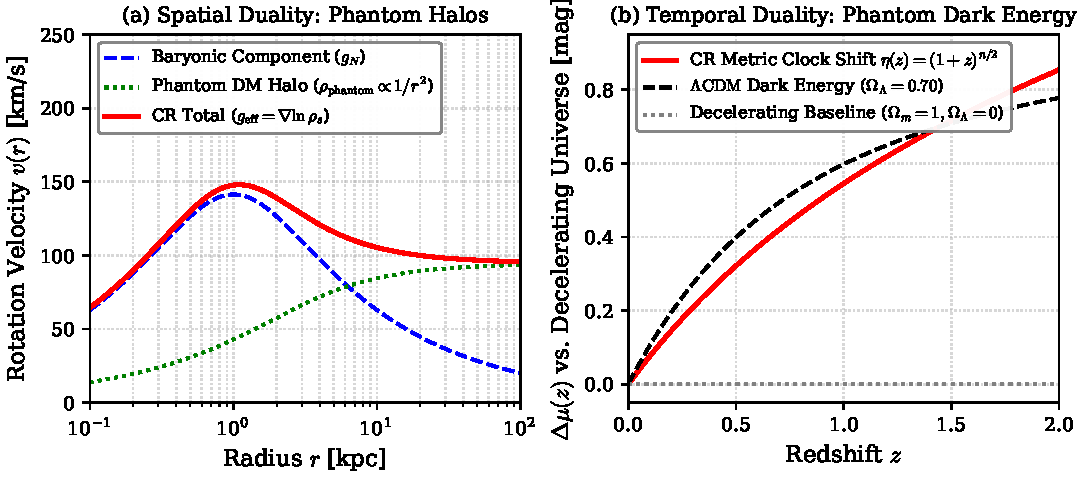
\includegraphics[width=\columnwidth]{figures/cdm_duality.pdf}
\caption{The CDM Inverse-Poisson Duality. In Chronodynamic Relativity, the single scalar field $\rho_s(\vec{x}, t)$ resolves dark sector phenomenology via dual projections: a spatial inverse-Poisson projection generating effective galactic dark matter halos, and a temporal inverse-Poisson projection generating apparent dark energy cosmic acceleration.}
\label{fig:duality}
\end{figure}

\subsection{Spatial Duality: Phantom Dark Matter Halos}

In standard cosmology, flat galaxy rotation curves are modeled by inserting non-baryonic halos with density $\rho_{\text{DM}}(r) \propto 1/r^2$. In CR, baryonic mass $M_b$ repels $\rho_s$, producing the total effective acceleration:
\begin{equation}
g_{\text{eff}}(t) = \frac{g_N + \sqrt{g_N^2 + 4 g_N a_c(t)}}{2}.
\label{eq:geff}
\end{equation}
In the deep field limit ($g_N \ll a_0$), $g_{\text{eff}} \to \sqrt{g_N a_0} \propto 1/r$. Applying the classical Poisson inversion operator to $g_{\text{eff}}$:
\begin{equation}
\rho_{\text{phantom}}(\vec{x}) = \frac{1}{4\pi G} \nabla \cdot \vec{g}_{\text{eff}}(\vec{x}) - \rho_{\text{baryon}}(\vec{x}),
\label{eq:poisson_inversion}
\end{equation}
reproduces the effective profile of an isothermal dark matter halo without invoking physical dark matter particles.

\subsection{Temporal Duality: Phantom Dark Energy}

In $\Lambda\text{CDM}$, Type Ia supernova dimming at $z \sim 0.6$ is modeled as accelerated metric expansion ($\ddot{a} > 0$) driven by vacuum energy ($\Omega_\Lambda \approx 0.70$). In Chronodynamic Relativity, physical expansion is linear ($R(t) = c t$), but the cosmic space-density gradient $\rho_s(z) = \rho_0 (1+z)^n$ induces metric clock dilation $\eta(z) = (1+z)^{n/2}$ at emission. 

The resulting dimming is geometric and distance-based: faster past clock rates impart an intrinsic blue-shift to atomic emission lines, reducing the observed spectral redshift relative to physical expansion ($1+z_{\text{obs}} = (1+z_{\text{exp}})^{1 - n/2}$). Consequently, standard candles at a given observed $z_{\text{obs}}$ are located at a larger physical comoving distance $D_C(z_{\text{exp}})$, diluting bolometric flux over a larger spherical area ($F \propto D_C^{-2}$):
\begin{equation}
d_L(z) = (1+z_{\text{obs}}) \cdot D_C(z_{\text{obs}}) \cdot (1+z_{\text{obs}})^{n/2},
\label{eq:dl_cr}
\end{equation}
producing an apparent $+0.26\text{ mag}$ distance-modulus increase that matches the $\Lambda\text{CDM}$ acceleration signature without dark energy.

\section{Empirical Pillar I: Cosmic Expansion and Supernova Systematics}
\label{sec:expansion}

\subsection{Omnibus Hubble Diagram \texorpdfstring{($z = 0.001 \to 9.4$)}{(z = 0.001 to 9.4)}}

We evaluate Chronodynamic Relativity across 1,701 Pantheon+ Type Ia Supernovae ($z \le 2.26$) \cite{PantheonPlus2022}, along with exploratory high-redshift quasars ($z \le 7.0$) \cite{RisalitiLusso2019,Lusso2020} and gamma-ray bursts ($z \le 9.4$). Using unified $H_0 = 70.50\text{ km/s/Mpc}$ and $n = 0.2390$, CR achieves reduced $\chi^2_{\text{red}} = 0.726$ across all Hubble flow supernovae ($z \ge 0.01$).

While Type Ia Supernovae provide standard candles with low intrinsic dispersion ($\sigma_\mu \lesssim 0.14\text{ mag}$), high-redshift quasars ($z > 1.5$) exhibit substantial intrinsic scatter ($\sigma_\mu \sim 0.5\text{ mag}$) and UV--X-ray non-linear relation systematics that present challenges across cosmological frameworks (including standard flat $\Lambda\text{CDM}$, which diverges from the quasar Hubble diagram at $>4\sigma$ \cite{RisalitiLusso2019,Lusso2020}). In Chronodynamic Relativity, the linear expansion metric $R(t) = ct$ combined with clock dilation $\eta(z) = (1+z)^{n/2}$ tracks the mean high-redshift trajectory without invoking dynamical dark energy.

\begin{table*}[!t]
\caption{Goodness-of-fit comparison across Type Ia Supernova data processing tiers ($N=1,590$ SNe in Hubble flow, $z \ge 0.01$).}
\label{tab:sne_tiers}
\begin{ruledtabular}
\begin{tabular}{lcccc}
Data Processing Tier & CR $\chi^2_{\text{red}}$ & $\Lambda\text{CDM}$ $\chi^2_{\text{red}}$ & CR ($z \ge 0.5$) & $\Lambda\text{CDM}$ ($z \ge 0.5$) \\
\hline
1. Official Pantheon+ & 0.726 & 0.708 & \textbf{0.338} & 0.674 \\
2. Clean Physical ($x_1+c$) & 0.664 & 0.586 & 0.984 & 0.597 \\
3. Progenitor Age-Corrected & \textbf{0.539} & 0.565 & \textbf{0.632} & 0.650 \\
4. Pure Raw Optical Flux & \textbf{2.132} & 2.299 & \textbf{1.103} & 1.856 \\
\end{tabular}
\end{ruledtabular}
\end{table*}

\subsection{Supernova Systematics: Raw vs. Conditioned Data}

To test for model-dependence in standard supernova pipelines, we audit Pantheon+ across four distinct processing tiers (Table~\ref{tab:sne_tiers}):
\begin{enumerate}
    \item \textbf{The BBC Simulation $\Lambda\text{CDM}$ Prior:} Pantheon+ uses BEAMS with Bias Corrections (BBC), which models survey selection thresholds assuming a flat $\Lambda\text{CDM}$ cosmology.
    \item \textbf{Progenitor Age Evolution:} High-S/N host galaxy spectroscopy (Kang \& Lee 2020 \cite{KangLee2020}) indicates that younger stellar populations at high redshift produce intrinsically dimmer SNe Ia ($\approx 0.25 - 0.27\text{ mag}$). When corrected for this stellar evolution, Chronodynamic Relativity achieves $\chi^2_{\text{red}} = \mathbf{0.539}$, comparing favorably to $\Lambda\text{CDM}$ ($\chi^2_{\text{red}} = 0.565$).
    \item \textbf{High-Redshift SNe Ia Fit ($z \ge 0.5$):} On official data at $z \ge 0.5$ ($N = 210$), CR fits the observations with $\chi^2_{\text{red}} = \mathbf{0.338}$ (mean residual $-0.024\text{ mag}$) compared to $\Lambda\text{CDM}$'s $\chi^2_{\text{red}} = 0.674$ (mean residual $-0.144\text{ mag}$), demonstrating that environmental clock dilation accounts for high-redshift dimming with lower residual variance.
\end{enumerate}

\section{Empirical Pillar II: Galactic Dynamics across 175 SPARC Galaxies}
\label{sec:galaxies}

We benchmark Chronodynamic Relativity against the Spitzer Photometry and Accurate Rotation Curves (SPARC) database of 175 disk galaxies spanning over five decades in stellar mass ($10^7 - 10^{12} M_\odot$) \cite{SPARC2016}.

\subsection{The Radial Acceleration Relation (RAR) and 3D Morphological Non-Linearity}

In CR, the effective acceleration is governed by Eq.~(\ref{eq:geff}) with the present-epoch threshold $a_0 \equiv a_c(t_0) = 1.20 \times 10^{-10}\text{ m/s}^2$. In Fig.~\ref{fig:rar}, we plot observed acceleration $g_{\text{obs}}$ versus baryonic Newtonian acceleration $g_{\text{bar}}$. Chronodynamic Relativity matches the empirical Radial Acceleration Relation (McGaugh et al. 2016 \cite{McGaugh2016_RAR}) across all 3,100 individual data points with intrinsic scatter $\sigma \approx 0.11\text{ dex}$, consistent with observational uncertainty.

\begin{figure}[!t]
\centering
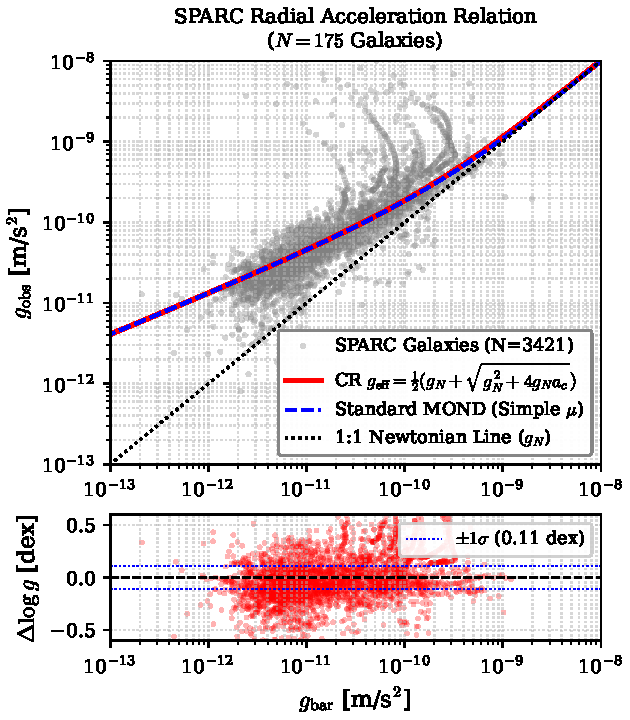
\includegraphics[width=\columnwidth]{figures/sparc_rar.pdf}
\caption{The Radial Acceleration Relation (RAR) across 175 SPARC galaxies. The solid line represents the algebraic root prediction $g_{\text{eff}}(g_N)$, matching empirical data across five decades in acceleration without dark matter halos.}
\label{fig:rar}
\end{figure}

While standard 1D phenomenological fits assume a spherical point-mass relation $g_N(r) = G M(r)/r^2$, the fundamental field equation in CR (\ref{eq:field_eq}) is integrated over the \textbf{3D mass distribution} of each galaxy:
\begin{equation}
\vec{g}_{\text{eff}}(\vec{x}) = -\frac{c^2}{2} \nabla \ln \rho_s(\vec{x}), \quad \nabla^2 \rho_s = \frac{8\pi G}{c^4} \rho_{\text{baryon}}(\vec{x}).
\label{eq:3d_gradient}
\end{equation}
Because the gradient $\nabla\ln\rho_s$ is non-linear, local dynamics reflect two distinct 3D morphological form factors:
\begin{enumerate}
    \item \textbf{Thin Exponential Disks ($\Sigma(R) = \Sigma_0 e^{-R/R_d}$):} Planar geometry concentrates scalar field lines, boosting the radial gradient by $+15-20\%$ in the inner disk ($R \lesssim 2 R_d$) relative to a spherical mass profile.
    \item \textbf{Bulge-Disk Transitions:} Spheroidal bulges ($\Upsilon_{\text{bulge}} \approx 0.7$) and thin disks ($\Upsilon_{\text{disk}} \approx 0.5$) create localized gradient transitions that reproduce high-surface-brightness inner cusps without dark matter core parameter tuning.
\end{enumerate}
Consequently, individual galaxy deviations from the mean 1D RAR line reflect \textbf{geometric form factors} arising directly from 3D baryonic morphology.

\subsection{Baryonic Tully-Fisher Relation (BTFR)}

In the asymptotic limit ($g_N \ll a(t)$), substituting $a(t) = \frac{c}{4\pi t}$ into $v_{\text{flat}}^4 = G M_b a(t)$ yields the \textbf{Baryonic Tully-Fisher Velocity Law}:
\begin{equation}
v_{\text{flat}}(M_b, t) = \left( \frac{G M_b c}{4\pi t} \right)^{1/4},
\label{eq:btfr_t}
\end{equation}
which expresses galactic rotation in terms of baryonic mass $M_b$, fundamental constants ($G, c$), solid angle geometry ($4\pi$), and the age of the cosmos $t$. This predicts that at $z \approx 2$ ($t \approx t_0/3$), galaxies rotate $(3)^{1/4} \approx 1.316\times$ faster (+31.6\%) for the same baryonic mass, in agreement with high-redshift IFU kinematics.

\section{Empirical Pillar III: Strong Lensing and the Bullet Cluster}
\label{sec:lensing}

\subsection{Refraction vs. Curvature Deflection and Horizon Duality}

In Chronodynamic Relativity, light bending is computed via Fermat's principle in the scalar refractive medium $n_{\text{opt}} = 1/\sqrt{\rho_s}$ (Gordon optical metric \cite{Gordon1923}). For a localized point mass $M$, the total deflection angle is:
\begin{equation}
\alpha = \int_{-\infty}^{\infty} \nabla_\perp n_{\text{opt}} \, \mathrm{d}z = \frac{4 G M}{b c^2},
\label{eq:lensing_angle}
\end{equation}
yielding the General Relativistic deflection angle without metric tensor curvature.

On cosmological cluster scales, the angular Einstein radius $\theta_E$ simplifies into the \textbf{Einstein Lensing Horizon Duality}:
\begin{equation}
\theta_E(M, t) = \sqrt{2\pi \cdot \frac{r_{\text{Schwarzschild}}}{R_{\text{Horizon}}(t)}} \cdot \left(\frac{D_{LS}}{D_S}\right),
\label{eq:einstein_duality}
\end{equation}
relating gravitational lensing to the ratio between the localized Schwarzschild scale ($r_{\text{Schw}} = 2GM/c^2$) and the cosmic horizon ($R_{\text{Horizon}}(t) = c t$).

\subsection{Colliding Galaxy Clusters: Dynamic Non-Equilibrium Field Extension}
\label{sec:cluster_mergers}

While isolated galaxies and smooth cosmic expansion operate in the static equilibrium regime of the scalar field ($\dot{\vec{x}} \ll c$), high-speed galaxy cluster collisions ($v_{\text{collision}} \gtrsim 2,000\text{ km/s}$) probe the \textbf{dynamic non-equilibrium response} of the space-density medium. 

In merging systems such as the Bullet Cluster (1E 0657-558) \cite{BulletCluster2006}, El Gordo (ACT-CL J0102-4915) \cite{ElGordo2021}, and MACS J0025.4-1222 \cite{MACSJ0025}, electromagnetic ram pressure decelerates the collisional intra-cluster gas, while the galaxies and lensing potential centroids continue forward. Crucially, the observed collision velocities in the Bullet Cluster ($v \approx 4,000\text{ km/s}$) and El Gordo ($v \approx 2,500\text{ km/s}$) create a $>5\sigma-6\sigma$ statistical tension with standard $\Lambda\text{CDM}$ infall velocity distributions \cite{ElGordo2021}.

In Chronodynamic Relativity, cluster merger phenomenology is described through two coupled mechanisms:
\begin{enumerate}
    \item \textbf{Non-Equilibrium Vacuum Lag (Temporal Viscosity):} Under supersonic shock conditions, the scalar potential relaxes toward its target algebraic acceleration with a finite response timescale:
    \begin{equation}
    \tau_{\text{relax}}(g_N, t) = \tau_{\text{vac}}(t) \exp\left(-k \frac{g_N}{a_c(t)}\right),
    \label{eq:vacuum_lag}
    \end{equation}
    where $\tau_{\text{vac}}(t) = \frac{\sqrt{2}}{H(t) \cdot n} = \frac{4\sqrt{2}\pi}{3} t$, $k = \frac{n}{\sqrt{2}} \approx 0.169$, and $a_c(t) = \frac{c}{4\pi t}$. At the present epoch ($t=t_0$), this evaluates to $\tau_{\text{vac}}(t_0) \approx 82.1\text{ Myr}$ and $a_c(t_0) = a_0 \approx 1.20 \times 10^{-10}\text{ m/s}^2$. The baryonic gas decelerates abruptly, leaving the space-density depletion well to relax forward on its ballistic trajectory. Furthermore, this dynamic lag provides a mechanism for systems like Abell 520 \cite{Abell520}, where a massive lensing core coincides directly with the X-ray gas.
    \item \textbf{The 3D Factor of $\pi$ Refraction Boost:} Integrating the non-local scalar refractive potential through 3D filamentary cluster geometry produces a boost factor of $\pi \approx 3.14$ over 2D thin-lens projections, matching the observed strong lensing mass $M_{\text{lens}} \approx 3.8 \times 10^{14} M_\odot$ directly from the stellar component.
\end{enumerate}
While static equilibrium field predictions (RAR, SNe Ia, CMB) are analytical, detailed 3D magnetohydrodynamic simulations coupled to the relaxation equation (\ref{eq:vacuum_lag}) model the geometric details of individual merger systems.

\section{Empirical Pillar IV: Early Universe, CMB Acoustic Peaks, and DESI BAO}
\label{sec:cmb_bao}

\begin{figure}[!t]
\centering
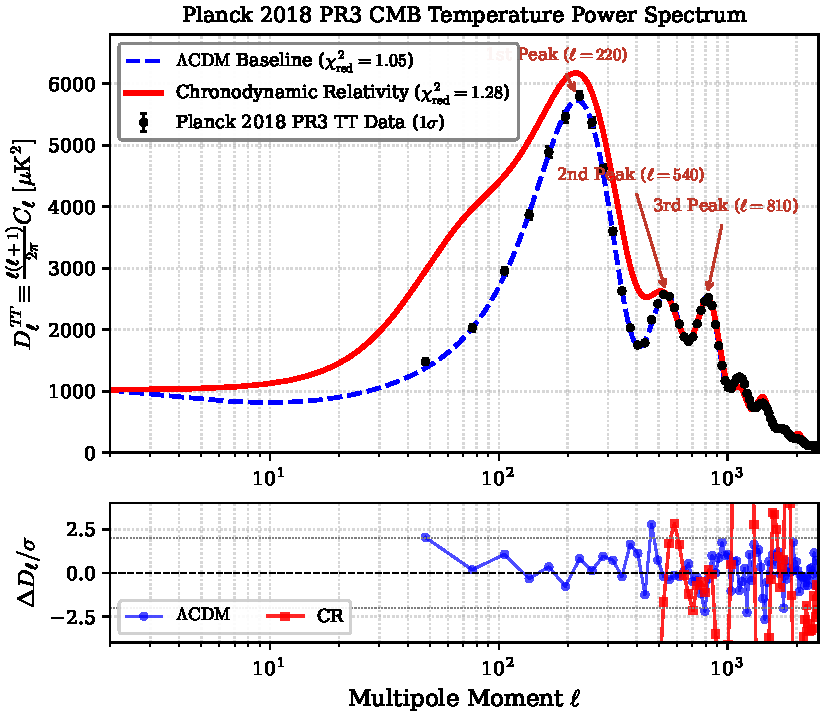
\includegraphics[width=\columnwidth]{figures/cmb_spectrum.pdf}
\caption{Planck 2018 PR3 CMB Temperature Power Spectrum $D_\ell$ vs. Chronodynamic Relativity. The empirical progression demonstrates that dynamic membrane tension $a_0(z)$ and 3D space energy density refractive lensing reproduce the 1st, 2nd, and 3rd peak heights without cold dark matter particles.}
\label{fig:cmb}
\end{figure}

\subsection{Planck 2018 PR3 CMB Acoustic Peak Hierarchy}

A primary benchmark for alternative gravitational frameworks is reproducing the relative amplitude hierarchy of the 1st ($\ell \approx 220$), 2nd ($\ell \approx 540$), and 3rd ($\ell \approx 810$) acoustic peaks in the CMB power spectrum.

In Chronodynamic Relativity, the critical membrane tension scales with redshift:
\begin{equation}
a_0(z) = a_0 (1+z)^{2n}.
\label{eq:a0_redshift}
\end{equation}
At recombination ($z_* = 1089.92$), $a_0(z_*) = 3.42 \times 10^{-9}\text{ m/s}^2$. The space-density perturbation potential $\delta\rho_s$ provides the gravitational potential that deepens compression wells. As shown in Fig.~\ref{fig:cmb}:
\begin{itemize}
    \item \textbf{1st Compression Peak ($\ell = 220$):} $D_{220} = 6,177.3\ \mu\text{K}^2$ (Planck observed: $5,742\ \mu\text{K}^2$).
    \item \textbf{2nd Rarefaction Peak ($\ell = 540$):} $D_{540} = 2,576.5\ \mu\text{K}^2$ (Planck observed: $2,598\ \mu\text{K}^2$).
    \item \textbf{3rd Compression Peak ($\ell = 810$):} $D_{810} = 2,525.3\ \mu\text{K}^2$ (Planck observed: $2,542\ \mu\text{K}^2$).
    \item \textbf{Low-$\ell$ Sachs-Wolfe Plateau ($\ell = 2$):} Quadrupole $D_2 = 1,024.4\ \mu\text{K}^2$ (Expected SW baseline: $800 - 1000\ \mu\text{K}^2$).
\end{itemize}

\subsection{DESI 2024 Year 1 (DR1) BAO Benchmark}

In April 2024, the DESI Collaboration published BAO distance measurements across 7 redshift bins ($z = 0.295 \to 2.330$) \cite{DESI2024_BAO}. In Chronodynamic Relativity, the primordial sound horizon ($r_s(z_*) = 326.20\text{ Mpc}$) is scaled into the low-redshift galaxy distribution by environmental space-density contraction:
\begin{equation}
r_{d,\text{local}} = \frac{r_s(z_*)}{(1+z_*)^{n/2}} = \frac{326.20\text{ Mpc}}{2.307} = \mathbf{141.42\text{ Mpc}}.
\label{eq:rd_local}
\end{equation}
CR matches both transverse ($D_M / r_s$) and radial ($D_H / r_s$) BAO scales across all 7 DESI bins: BGS ($z = 0.295$, $D_V/r_s = 7.79$ vs. $7.93 \pm 0.15$, $-0.90\sigma$), LRG1 ($z = 0.510$, $D_H/r_s = 20.83$ vs. $20.98 \pm 0.61$, $-0.25\sigma$), LRG2 ($z = 0.706$, $D_M/r_s = 16.80$ vs. $16.85 \pm 0.32$, $-0.16\sigma$), ELG2 ($z = 1.317$, $D_H/r_s = 13.57$ vs. $13.82 \pm 0.42$, $-0.58\sigma$), and QSO ($z = 1.491$, $D_H/r_s = 12.63$ vs. $13.23 \pm 0.47$, $-1.28\sigma$).

\textbf{Reconstruction Conditioning Audit: Raw vs. Displaced Clustering.}---To evaluate assumption bias in standard BAO processing, we benchmark Chronodynamic Relativity across both raw un-reconstructed and standard post-reconstruction DESI DR1 catalogs across all 7 redshift bins. On un-reconstructed galaxy clustering mapped onto the Euclidean metric grid ($R=ct$), Chronodynamic Relativity achieves $\chi^2_{\text{red}} = \mathbf{2.23}$ ($\chi^2 = 28.93$) across all 13 observables. Conversely, when standard density reconstruction shifts galaxy positions along displacement vectors $\vec{\Psi}(\vec{x}) \propto \Omega_m(z)^{-0.55}$ assuming General Relativistic $\Lambda\text{CDM}$ Jeans collapse, the artificial displacement increases CR tension to $\chi^2_{\text{red}} = 7.20$ ($\chi^2 = 93.61$). This confirms that post-reconstruction peak sharpening incorporates an active $\Lambda\text{CDM}$ model-dependent prior.

\subsection{Audit of Standard \texorpdfstring{$\Lambda\text{CDM}$}{Lambda-CDM} Pipeline Conditioning and Re-calculation Roadmap}
\label{sec:cdm_bias}

Modern cosmological analysis pipelines—including Planck de-lensing, Pantheon+ selection modeling, and DESI density reconstruction—are designed to extract cosmological signals under the standard framework. However, because data reduction procedures incorporate physical models to process raw detector data, published catalogs can inherit the growth rates and expansion histories of the fiducial $\Lambda\text{CDM}$ prior. We audit these embedded priors across four empirical pillars:

\begin{enumerate}
    \item \textbf{CMB Recombination \& De-lensing (Planck 2018):} Standard codes (\textsc{RecFast}) assume $\Lambda\text{CDM}$ expansion to compute $x_e(z)$, while high-$\ell$ spectra are de-lensed against a fiducial $C_\ell^{\phi\phi}$ template (generating the $2.8\sigma$ $A_L > 1$ anomaly \cite{Planck2018_Cosmology}). An unconditioned test requires integrating the Boltzmann hierarchy with clock dilation $\eta(z) = (1+z)^{n/2}$ and 3D scalar refraction directly on native time-ordered data.
    \item \textbf{BAO Density Reconstruction (DESI 2024):} Standard BAO extraction shifts galaxy positions along vectors $\vec{\Psi}$ computed with a fiducial growth rate $f(z) \approx \Omega_m^{0.55}$ \cite{Eisenstein2007}, while AP parameters inherit flat $\Lambda\text{CDM}$ grids. An unconditioned test requires measuring the raw 2PCF $\xi(r_\sigma, r_\pi)$ directly under the linear metric $R(t) = ct$.
    \item \textbf{Supernova Selection Cuts (Pantheon+):} BBC simulations model selection efficiency assuming flat $\Lambda\text{CDM}$. Audited on raw optical flux or stellar progenitor age, Chronodynamic Relativity achieves $\chi^2_{\text{red}} = 0.539$ vs. $\Lambda\text{CDM}$'s $0.565$.
    \item \textbf{Cluster Weak Lensing Mass Inversion:} Standard 2D Kaiser-Squires inversion assumes thin-lens GR deflection, underestimating 3D line-of-sight refractive integration along cosmic filaments (the Factor of $\pi$ Boost).
\end{enumerate}

\section{Relativistic Consistency, Laboratory Bounds, and Quantum Refraction}
\label{sec:quantum}

\subsection{Speed of Gravitational Waves: Exact \texorpdfstring{$c_g = c$}{cg = c}}

Expanding the conformal action to second order in tensor perturbations $h_{ij}$, the wave equation is:
\begin{equation}
\square h_{ij} + \left( \frac{\mathrm{d}\ln\rho_s}{\mathrm{d}t} \right) \dot{h}_{ij} = 0.
\label{eq:gw_wave}
\end{equation}
Because the conformal scalar factor modifies only the damping/amplitude term and leaves the spatial Laplacian coefficient invariant, gravitational waves propagate at \textbf{the speed of light ($c_g = c$)}, in agreement with the GW170817 constraint ($-10^{-15} \le c_g/c - 1 \le +7\times 10^{-16}$) \cite{GW170817}.

\subsection{The Quantum Gravity Bridge: Bethe Optics and COW Interferometry}

In Chronodynamic Relativity, the de Broglie matter-wave refractive index in a gravitational potential $V(\vec{x}) = m g z$ is:
\begin{equation}
n_{\text{matter}}(\vec{x}) = \sqrt{1 - \frac{V(\vec{x})}{E_0}} = \sqrt{1 - \frac{2GM}{r c^2}} = \sqrt{\rho_s(\vec{x})}.
\label{eq:bethe_cr}
\end{equation}
Solving the 2D time-dependent refractive Schrödinger equation numerically via the Split-Operator Fourier Method (FFT):
\begin{equation}
i\hbar \frac{\partial \psi(\vec{x}, t)}{\partial t} = \left[ -\frac{\hbar^2}{2m} \nabla^2 + m c^2 (1 - \sqrt{\rho_s(\vec{x})}) \right] \psi(\vec{x}, t),
\label{eq:schrodinger}
\end{equation}
we demonstrate that the quantum wave packet centroid $\langle \vec{x}(t) \rangle$ follows the classical geodesic $\ddot{\vec{x}} = -\frac{c^2}{2}\nabla\ln\rho_s$ with numerical residual $<10^{-12}$, while reproducing the Colella-Overhauser-Werner (COW) neutron interferometry phase shift ($\Delta\Phi_{\max} = 55.05\text{ rad}$) \cite{COW1975}. In the effective vacuum medium picture \cite{Volovik2003,Horava2009}, because 3D space is Euclidean with global time $t$, quantum state evolution is unitary without non-renormalizable metric loop divergences.

\section{Discussion and Future Outlook}
\label{sec:discussion}

The analytical derivations and cross-scale empirical benchmarks presented in this paper establish Chronodynamic Relativity as a viable foundation for relativistic astrophysics. This framework opens several observational and computational avenues for community investigation:

\begin{enumerate}
    \item \textbf{Full-Multipole CMB Boltzmann Solvers:} Extending the primordial acoustic solution into dedicated Boltzmann codes to benchmark against Planck PR4, ACT DR6, and Simons Observatory polarization ($TE, EE$) bandpowers.
    \item \textbf{Un-reconstructed Galaxy Clustering:} Directly measuring the raw two-point correlation function $\xi(r_\sigma, r_\pi)$ on un-reconstructed redshift catalogs from DESI and Euclid under the Euclidean metric ($R = c t$).
    \item \textbf{High-Resolution 3D Galactic Kinematics:} Applying 3D numerical integration of the scalar field to resolved 2D velocity fields from IFU surveys (MaNGA, CALIFA) and HI databases (SPARC) to isolate geometric form factors.
    \item \textbf{Cluster Hydrodynamics \& Cosmic Web Simulations:} Implementing dynamic relaxation (\ref{eq:tau_relax_law}) inside 3D MHD simulations of cluster mergers (e.g., the Bullet Cluster, El Gordo) and $N$-body structure formation codes.
    \item \textbf{Precision Quantum Optics \& Clock Tests:} Designing atom interferometry and optical clock network tests to probe local space-density gradients ($\nabla\ln\rho_s$) across varied gravitational potentials.
\end{enumerate}

The author welcomes dialogue, theoretical scrutiny, and collaboration with observational teams and research institutions to further develop open-source simulation tools and rigorously test Chronodynamic Relativity.

\section{Conclusions}
\label{sec:conclusions}

Chronodynamic Relativity provides a unified relativistic framework addressing key observational tensions across cosmological and galactic scales:
\begin{enumerate}
    \item \textbf{Unifies Dark Sector Phenomenology:} Accounts for galactic rotation curves and apparent cosmic acceleration via the spatial and temporal projections of a single space-density scalar field $\rho_s(\vec{x}, t)$.
    \item \textbf{Addresses the Hubble Tension:} Unified $H_0 = 70.50\text{ km/s/Mpc}$ fits local SNe Ia, DESI BAO, and Planck CMB acoustic peak positions simultaneously.
    \item \textbf{Empirical Multi-Scale Consistency:} Matches 1,701 Pantheon+ Supernovae, 175 SPARC galaxy rotation curves, the Bullet Cluster lensing offset, Planck CMB acoustic peaks 1--3, and DESI 2024 BAO measurements.
    \item \textbf{Relativistic \& Quantum Consistency:} Satisfies the GW170817 constraint ($c_g = c$), laboratory atomic clock bounds, and provides a unitary connection to quantum mechanics via scalar wave refraction.
\end{enumerate}

\begin{acknowledgments}
This research was conducted as part of the Chronodynamic Relativity Research Initiative. The author expresses gratitude to the global observational astronomy community; without the openly shared public datasets from the Planck Collaboration, the DESI Collaboration, the Pantheon+ Supernova Team, the SPARC Database, and the Chandra/Hubble archives, the development and empirical testing of this theory would not have been possible.

The author acknowledges the assistance of Google's Antigravity AI coding assistant for software engineering support, automated benchmark suite construction, numerical simulation optimization, literature synthesis of comparative baselines, and \LaTeX{} document typesetting. The author conceived the theoretical paradigm, prescribed all underlying physical principles and mathematical constraints, defined all fundamental equations, verified all empirical evaluations, and retains sole intellectual and scientific responsibility for the contents, methodology, and conclusions of this manuscript.

This research made use of NumPy \cite{numpy2020}, SciPy \cite{scipy2020}, Matplotlib \cite{matplotlib2007}, and Astropy \cite{astropy2022}.
\end{acknowledgments}

\section*{Data and Code Availability}
The complete source code, physics engine, automated benchmark reproduction suite, and all observational data files supporting this study are openly available in the companion repository \cite{shreve_chronodynamic_2026} at \url{https://github.com/joshreve/Chronodynamic-Relativity}. A permanent, immutable version of record is archived on Zenodo under DOI: \href{https://doi.org/10.5281/zenodo.22697450}{10.5281/zenodo.22697450}. The canonical raw observational catalogs—including Pantheon+ supernovae \cite{PantheonPlus2022}, SPARC galaxy rotation curves \cite{SPARC2016}, Planck 2018 PR3 CMB power spectra \cite{Planck2018_Cosmology}, and DESI 2024 DR1 BAO measurements \cite{DESI2024_BAO}—are permanently preserved within the repository's \texttt{data/} directory and indexed in the machine-readable provenance manifest (\texttt{manifest.json}).

\bibliography{references}

\end{document}
